\documentclass[12pt,a4paper,utf8]{ctexart}
\usepackage{ctex,amsmath,amssymb,subfig,cite,graphicx,diagbox,fontspec,fancyhdr,geometry}
\usepackage[ntheorem]{empheq}
\usepackage{enumitem,fullpage,cleveref,cellspace,listings,color,framed}
\definecolor{gray}{rgb}{0.5,0.5,0.5}
\definecolor{dkgreen}{rgb}{.068,.578,.068}
\definecolor{dkpurple}{rgb}{.320,.064,.680}

%set Fortran styles
\lstset{
    frameround=tftf,
    language=Fortran,
    keywords={SELECT,PROGRAM,PRINT,STOP,END,WRITE,INTEGER,REAL,COMPLEX,CHARACTER,LOGICAL,READ,FORMAT,IMPLICIT,PARAMETER,DATA,EQUIVALENCE,TYPE,PAUSE,CONTINUE,CYCLE,EXIT,IF,SELECT,DO,ALLOCATE,DEALLOCATE,WHERE,FORALL,SUBROUTIHNE,CALL,RETURN,FUNCTION,COMMON,BLOCK DATA,SAVE,INTERFACE,CONTAIN,MODULE,USE,PUBLIC,PRIVATE,ENTRY,OPEN,INQUIRE,CLOSE,NAMELIST,POINTER,NULLFY,REWIND,BACKSPACE,ENDFILE
    },
    basicstyle=\small\ttfamily,
    numbers=left,
    numberstyle=\small,
    keywordstyle=\color{blue}\bfseries,
    commentstyle=\color{dkgreen},
    stringstyle=\color{dkpurple},
    backgroundcolor=\color{white},
    tabsize=2,
    showspaces=false,
    showstringspaces=false,
    breaklines=true,
    frame=trBL,
}
\CTEXsetup[format+={\raggedright}]{section}
\setlength{\parindent}{2em}
\geometry{
    textwidth=138mm,
    textheight=215mm,
    left=27mm,
    right=27mm,
    top=25.4mm,
    bottom=25.4mm,
    headheight=2.17cm,
    headsep=4mm,
    footskip=12mm,
    heightrounded,
}
\pagestyle{fancy}
\lhead{\textsl{2021秋-计算物理A}}
\chead{}
\rhead{\textsl{PB19020634-于浩然}}
\lfoot{}
\cfoot{\thepage}
\rfoot{}

\begin{document}
\begin{center}
    {\LARGE\textbf{计算物理作业五}}\\
    \textrm{于浩然}~~~~~~\textrm{PB19020634}~~~~~~\textrm{2021.10.17}
\end{center}

\section{作业题目}

对于球面上均匀分布的随机坐标点,给出它们在$(x,y)$平面上投影的几率密度分布函数.并由此验证Marsaglia抽样方法:
\begin{equation}
    x=2u \sqrt{1-r^2},\quad y=2v \sqrt{1-r^2}, \quad z=1-2r^2
\end{equation}
确为球面上均匀分布的随机抽样.

\section{算法简介}

\subsection{Marsaglia抽样方法}

\textsl{Marsaglia}抽样方法是一种由一对随机数序列 $(u,v) \in
[-1,1]$求三维球面上均匀分布点的方法,具体为:
\begin{enumerate}
    \item 随机抽样一对均匀分布的随机数 $(u,v) \in [-1,1]$;
    \item 计算 $r^2=u^2+v^2$,若$r^2 > 1 $则重新抽样直到 $r^2 \leq 1$;
    \item 得
        \begin{equation}
            x=2u \sqrt{1-r^2},\quad y=2v \sqrt{1-r^2}, \quad z=1-2r^2
        \end{equation}
\end{enumerate}  
\subsection{球面上均匀分布点在$(x,y)$平面上投影的几率密度分布函数}
首先定义球坐标系 $(\rho, \theta,
\varphi)$中单位球面上的“均匀分布”,可理解为在相同面积元 $
\textrm{d}S = \sin \theta \textrm{d} \theta \textrm{d} \varphi$上取点的概率 $ \textrm{d}P$均相同,可表达如下式:
\begin{equation}
    \textrm{d} P = p(\theta,\varphi) \textrm{d} \theta \textrm{d}
    \varphi = p(\theta,\varphi) \textrm{d}S / \sin \theta
\end{equation}
\begin{equation}
    \frac{ \textrm{d}P}{ \textrm{d}S} = \frac{p( \theta, \varphi)}{\sin \theta}
    = const.
\end{equation}

为满足上述关系,我们不妨设$p(\theta, \varphi) = k \sin \theta $ ($k$为常数)

对于球面有$0 \leq \theta \leq \pi $,$0 \leq \varphi
\leq 2\pi$由归一化关系:
\begin{equation}
    \iint p(\theta, \varphi) \textrm{d} \theta \textrm{d} \varphi = \int_0 ^{2
    \pi} \int _0 ^{\pi} k \sin \theta \textrm{d} \theta \textrm{d} \varphi =
   4\pi k =1
\end{equation}

因此我们得到$k=1/4\pi$,
\begin{equation}
p(\theta, \varphi)=\sin \theta / 4\pi
\end{equation}

设投影至$(x,y)$平面的几率密度分布函数为$f(x,y)$,$x=\sin \theta \cos
\varphi,y=\sin \theta \sin \varphi$,可得下式:
\begin{equation}
    f(x,y) \textrm{d}x \textrm{d}y = p(\theta, \varphi) \textrm{d} \theta \textrm{d} \varphi
\end{equation}
\begin{equation}
    f(x,y) \textrm{d}x \textrm{d}y = \frac{\sin \theta}{4\pi} \left |
    \frac{\partial (\theta,\varphi)}{\partial (x,y)} \right | \textrm{d}x \textrm{d}y
\end{equation}

其中
\begin{equation}
    \left |\frac{\partial (\theta,\varphi)}{\partial (x,y)} \right|
    =\left | \frac{\partial (x,y)}{\partial (\theta, \varphi)} \right |^{-1}
    = \frac{1}{\sin \theta \cos \theta}
\end{equation}

为Jacobi行列式.这样得到 $f(x,y)$(未归一化):
\begin{equation}
    f(x,y) = \frac{1}{4\pi} \frac{1}{\cos \theta} = \frac{1}{4\pi
    \sqrt{1-(x^2+y^2)}}
\end{equation}

由于将球面上点投影到坐标轴平面上时,上半球面和下半球面上的点都会被投影,概率密度函数
$f(x,y)$需要进行系数调整.设归一化的几率密度分布函数为
$g(x,y)=kf(x,y)$($k$为常数),考虑归一化条件:
\begin{eqnarray}
    & \. &\iint _{x^2+y^2 \leq 1} g(x,y) \textrm{d}x \textrm{d}y \nonumber \\
    &=& k\int _0 ^{2\pi} \int _0 ^1 \frac{r}{4\pi \sqrt{1-r^2}} \textrm{d}r
    \textrm{d}\varphi \nonumber \\
    &=& k\frac{1}{2} \int _0 ^1 \frac{r}{\sqrt{1-r^2}} \textrm{d}r \nonumber \\
    &=& \frac{k}{2} = 1 
\end{eqnarray}

因此,投影点的归一化的几率密度分布函数为:
\begin{equation}
    g(x,y) = \frac{1}{2\pi \sqrt{1-(x^2+y^2)}}
\end{equation}

\subsection{验证Marsaglia方法为球面上均匀分布的随机抽样}

对本题中的Marsaglia抽样方法,考察其坐标$(x,y)$的几率密度分布函数,若由我们上一节推出的函数式(12)把$(x,y)$的分布函数(1)变换到$(u,v)$的均匀分布,则可在一定程度上说明Marsaglia方法确为球面上均匀分布的随机抽样.

设几率密度分布函数$h(x,y),l(u,v)$,其中$l(u,v)$为均匀分布:
\begin{equation}
    l(u,v)=
    \begin{cases}
        1/4, \qquad -1 \leq u \leq 1, -1 \leq v \leq 1 \\
        0, \qquad otherwise
    \end{cases}
\end{equation}

有如下变换关系:
\begin{equation}
    l(u,v) \textrm{d}u \textrm{d}v = h(x,y) \textrm{d}x \textrm{d}y 
    = h(x,y) \left | \frac{\partial (x,y)}{\partial(u,v)} \right | \textrm{d}u
    \textrm{d}v
\end{equation}

其中Jacobi行列式:
\begin{equation}
    \left | \frac{\partial (x,y)}{\partial(u,v)} \right | = |4 - 8(u^2+v^2)|
\end{equation}
\begin{eqnarray}
    l(u,v) &=& h(x,y) \left | \frac{\partial (x,y)}{\partial(u,v)} \right |
    = \frac{|4-8(u^2+v^2)|}{2\pi \sqrt{1-(x^2+y^2)}} \nonumber \\
           &=& \frac{4|1-2(u^2+v^2)|}{2\pi \sqrt{1-4(u^2+v^2)[1-(u^2+v^2)]} }
           \nonumber \\
           &=& \frac{2}{\pi}  
\end{eqnarray}

这一分布函数正是$-1 \leq u \leq 1, -1 \leq v \leq
1$的均匀分布,与(13)式仅相差一个归一化系数.

为了保持严谨性,再证明Marsaglia抽样在$(x,z)$平面上的投影也满足(12).设$(x,z)$平面上投影的几率密度分布函数为$p(x,z)$.由(1)计算可得Jacobi行列式:
\begin{equation}
    \left | \frac{ \partial (x,z)}{\partial (u,v)} \right | = |8v
    \sqrt{1-(u^2+v^2)}|
\end{equation}

代入计算如下:
\begin{equation}
    l(u,v) \textrm{d}u \textrm{d}v = p(x,z) \left | \frac{\partial
    (x,z)}{\partial (u,v)} \right |\textrm{d}u \textrm{d}v
\end{equation}
\begin{eqnarray}
    l(u,v) &=& p(x,z) \left | \frac{\partial (x,z)}{\partial (u,v)} \right |
    \nonumber \\
           &=& \frac{8|v| \sqrt{1-(u^2+v^2)}}{2\pi \sqrt{1-(x^2+z^2)}} \nonumber
           \\
           &=& \frac{2}{\pi}
\end{eqnarray}

同理,这是一个均匀分布,Marsaglia抽样方法在$(x,z)$平面上的投影也与球面上均匀分布对应的投影相一致.同理我们可以得知$(y,z)$平面上的投影也是如此.Marsaglia抽样方法的结果在三个方向上投影的几率密度分布函数都与球面上真正均匀分布的密度函数一致,至此我们已经简略证明了Marsaglia抽样方法可以认为是球面上均匀分布的抽样.
\newpage
\section{编程实现}

前面已经在理论上证明了Marsaglia抽样方法的结果为球面上均匀分布,为了更直观的表述这一结果,使用Fortran90编程进行数值实验,并用python脚本绘图展示.
\begin{itemize}
    \item \texttt{PROGRAM MAIN}
    
    分别取$10^3,10^4,10^5$个点进行抽样,在主程序中通过
    \texttt{DO}语句实现.这里的随机数种子(6、7行)采用了最原始的办法,就是滚键盘.

\begin{framed}
\begin{lstlisting}[language=Fortran]
PROGRAM MAIN
    INTEGER(KIND=4) :: intI
    CHARACTER(LEN=1) :: charI
    DO intI = 3, 5
        WRITE (charI,"(I1)") intI !此语句将10以内的整型数据intI变为字符类型charI
        CALL Schrage(intI, 98456523,'u'//charI//'.dat')
        CALL Schrage(intI, 1654125, 'v'//charI//'.dat')
        CALL Marsaglia(intI) !由Marsaglia抽样方法从u,v抽出随机数点
    END DO
END PROGRAM MAIN
\end{lstlisting}
\end{framed}

\item \texttt{SUBROUTINE Schrage(P, z0, filename)}

    常规的16807生成器,传入参数可确定生成的随机数多少、种子和存放随机数序列的文件名
    \texttt{'*.dat'}.

\begin{framed}
\begin{lstlisting}[language=Fortran]
SUBROUTINE Schrage(P, z0, filename) !Schrage随机数生成器子程序
   IMPLICIT NONE
   INTEGER :: N = 1, P
   INTEGER :: m = 2147483647, a = 16807, q = 127773, r = 2836, In(10**P), z0
   REAL(KIND=8) :: z(10**P)
   CHARACTER(LEN=40) :: filename
   In(1) = z0 !将传入值z0作为种子
   z(1) = REAL(In(1))/m
   DO N = 1, 10**P - 1
      In(N + 1) = a*MOD(In(N), q) - r*INT(In(N)/q)
      IF (In(N + 1) < 0) THEN !若值小于零,按Schrage方法加m
         In(N + 1) = In(N + 1) + m
      END IF
      z(N + 1) = REAL(In(N + 1))/m !得到第N+1个随机数
   END DO
   OPEN (1, file=trim(filename)) !每次运行子程序按照传入参数filename生成数据文件
   DO N = 1, 10**P !将随机数按行存入文件
      WRITE (1, *) z(N)
   END DO
   CLOSE (1)
END SUBROUTINE Schrage
\end{lstlisting}
\end{framed}

\item \texttt{SUBROUTINE Marsaglia(intP)}

    传入参数 \texttt{intP}确定对多少随机数点进行抽样,读取
    \texttt{Schrage}子程序生成的随机数文件并将其转化为$[-1,1]$上的均匀分布随机数(见13、14行).当
    $u^2+v^2 <
    1$时按照公式(1)计算得到抽样值,而当$u^2+v^2>1$时不进行操作;由于被抽样点的个数决定于先前
    \texttt{Schrage}
    子程序所写的文件,最终抽样结果的点数随种子的改变而变化,大体上由抽样效率$\pi/4$决定.由于绘制图像时对点数的要求并不严格,这里采用了不确定总点数的方法.

\begin{framed}
\begin{lstlisting}[language=Fortran]
SUBROUTINE Marsaglia(intP)
    INTEGER(KIND=4) :: intP, i = 1, num
    CHARACTER(LEN=1) charP
    REAL(KIND=8), DIMENSION(10**intP) :: u, v
    REAL(KIND=8), DIMENSION(10**intP, 3) :: r !存放随机数点坐标的二维数组
    WRITE (charP,"(I1)") intP !将整型数据intP转为字符型数据charP
    OPEN (1, file='u'//charP//'.dat') !打开相应文件传入两组随机数序列
    READ (1, *) u
    CLOSE (1)
    OPEN (1, file='v'//charP//'.dat')
    READ (1, *) v
    CLOSE (1)
    u = 2 * u - 1
    v = 2 * v - 1
    num = 0 !初始化抽出点的个数
    DO i = 1, 10**intP !遍历被抽样的所有点
        IF (u(i)**2 + v(i)**2 <= 1) THEN !当u^2+v^2<1时抽样
            num = num + 1 !抽出点后总抽出点数num递增,并进行抽样运算
            r(num, 1) = 2 * u(i) * SQRT(1 - u(i)**2 - v(i)**2)
            r(num, 2) = 2 * v(i) * SQRT(1 - u(i)**2 - v(i)**2)
            r(num, 3) = 1 - 2 * (u(i)**2 + v(i)**2)
        ENDIF
    END DO
    OPEN (1, file='x'//charP//'.dat') !将x,y,z坐标分别存入相应文件
    DO i = 1, num
        WRITE (1, *) r(i, 1)
    END DO
    CLOSE (1)
    OPEN (1, file='y'//charP//'.dat') 
    DO i = 1, num
        WRITE (1, *) r(i, 2)
    END DO
    OPEN (1, file='z'//charP//'.dat') 
    DO i = 1, num
        WRITE (1, *) r(i, 3)
    END DO
END SUBROUTINE Marsaglia
\end{lstlisting}
\end{framed}

\item python绘图脚本

此脚本中只需改动几次文件名,便可依照我们之前所写的文件绘制三维空间中随机数点分布的散点图,绘图结果展示于下一部分.
\begin{framed}
\begin{lstlisting}[language=python]
import matplotlib.pyplot as plt
import numpy as np

plt.rcParams['savefig.dpi'] = 300  #设置输出图像分辨率
plt.rcParams['figure.dpi'] = 300

fig = plt.figure()
ax1 = plt.axes(projection='3d')

x = np.loadtxt("x4.dat")
y = np.loadtxt("y4.dat")
z = np.loadtxt("z4.dat")

ax1.scatter3D(x, y, z, s=1)
plt.gca().set_box_aspect(aspect=(1, 1, 1))  # 调整比例尺均匀
ax1.set_xlabel('x')
ax1.set_ylabel('y')
ax1.set_zlabel('z')
plt.savefig("fig4.eps")
\end{lstlisting}
\end{framed}
\end{itemize}

\section{计算结果}

对$10^3,10^4,10^5$个被抽样点,最终抽出的点数分别为779,7792,78375,与Marsaglia抽样方法的抽样效率$\pi/4
= 0.7854$
吻合.将这些抽样得到的点绘制3D散点图在下页展示,可以观察到,在点数较少时还可以观察出点集中分布的趋向,随着点数增多分布近乎均匀,直观地验证了Marsaglia抽样方法能够得到球面上均匀分布的随机数点.

\section{结论}

本题中我们推导了球面上均匀分布点投影在坐标平面上的几率密度分布函数,并通过数学上的推导比较初步确定了Marsaglia抽样方法是球面上均匀分布的随机抽样;随后我们编写程序实现Marsaglia方法,亲身实践了舍选抽样法算法的具体细节,能够成功实现对指定个数被抽点的抽样.本程序还可以进一步改善,实现给定抽出点数的抽样,这样可能会需要16807产生器产生大于这一数目的随机数序列.

\newpage

\begin{figure}[htb]
    \centering
    \subfloat[779个随机数点]{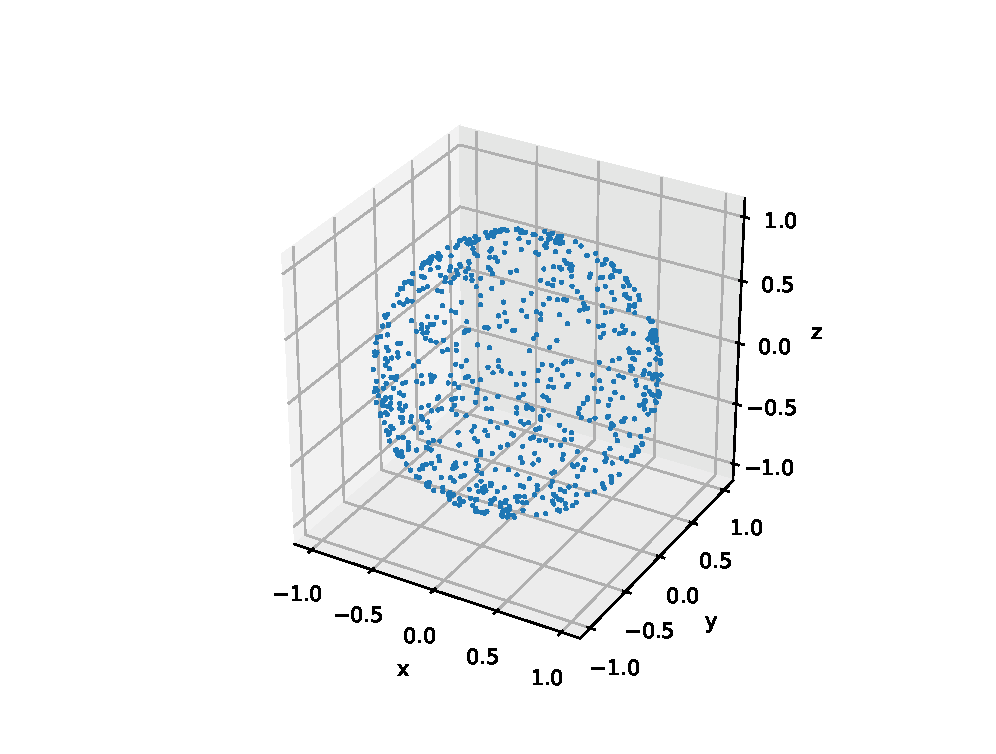
\includegraphics[width=0.48\textwidth]{fig3.eps}} \hfill
    \subfloat[7792个随机数点]{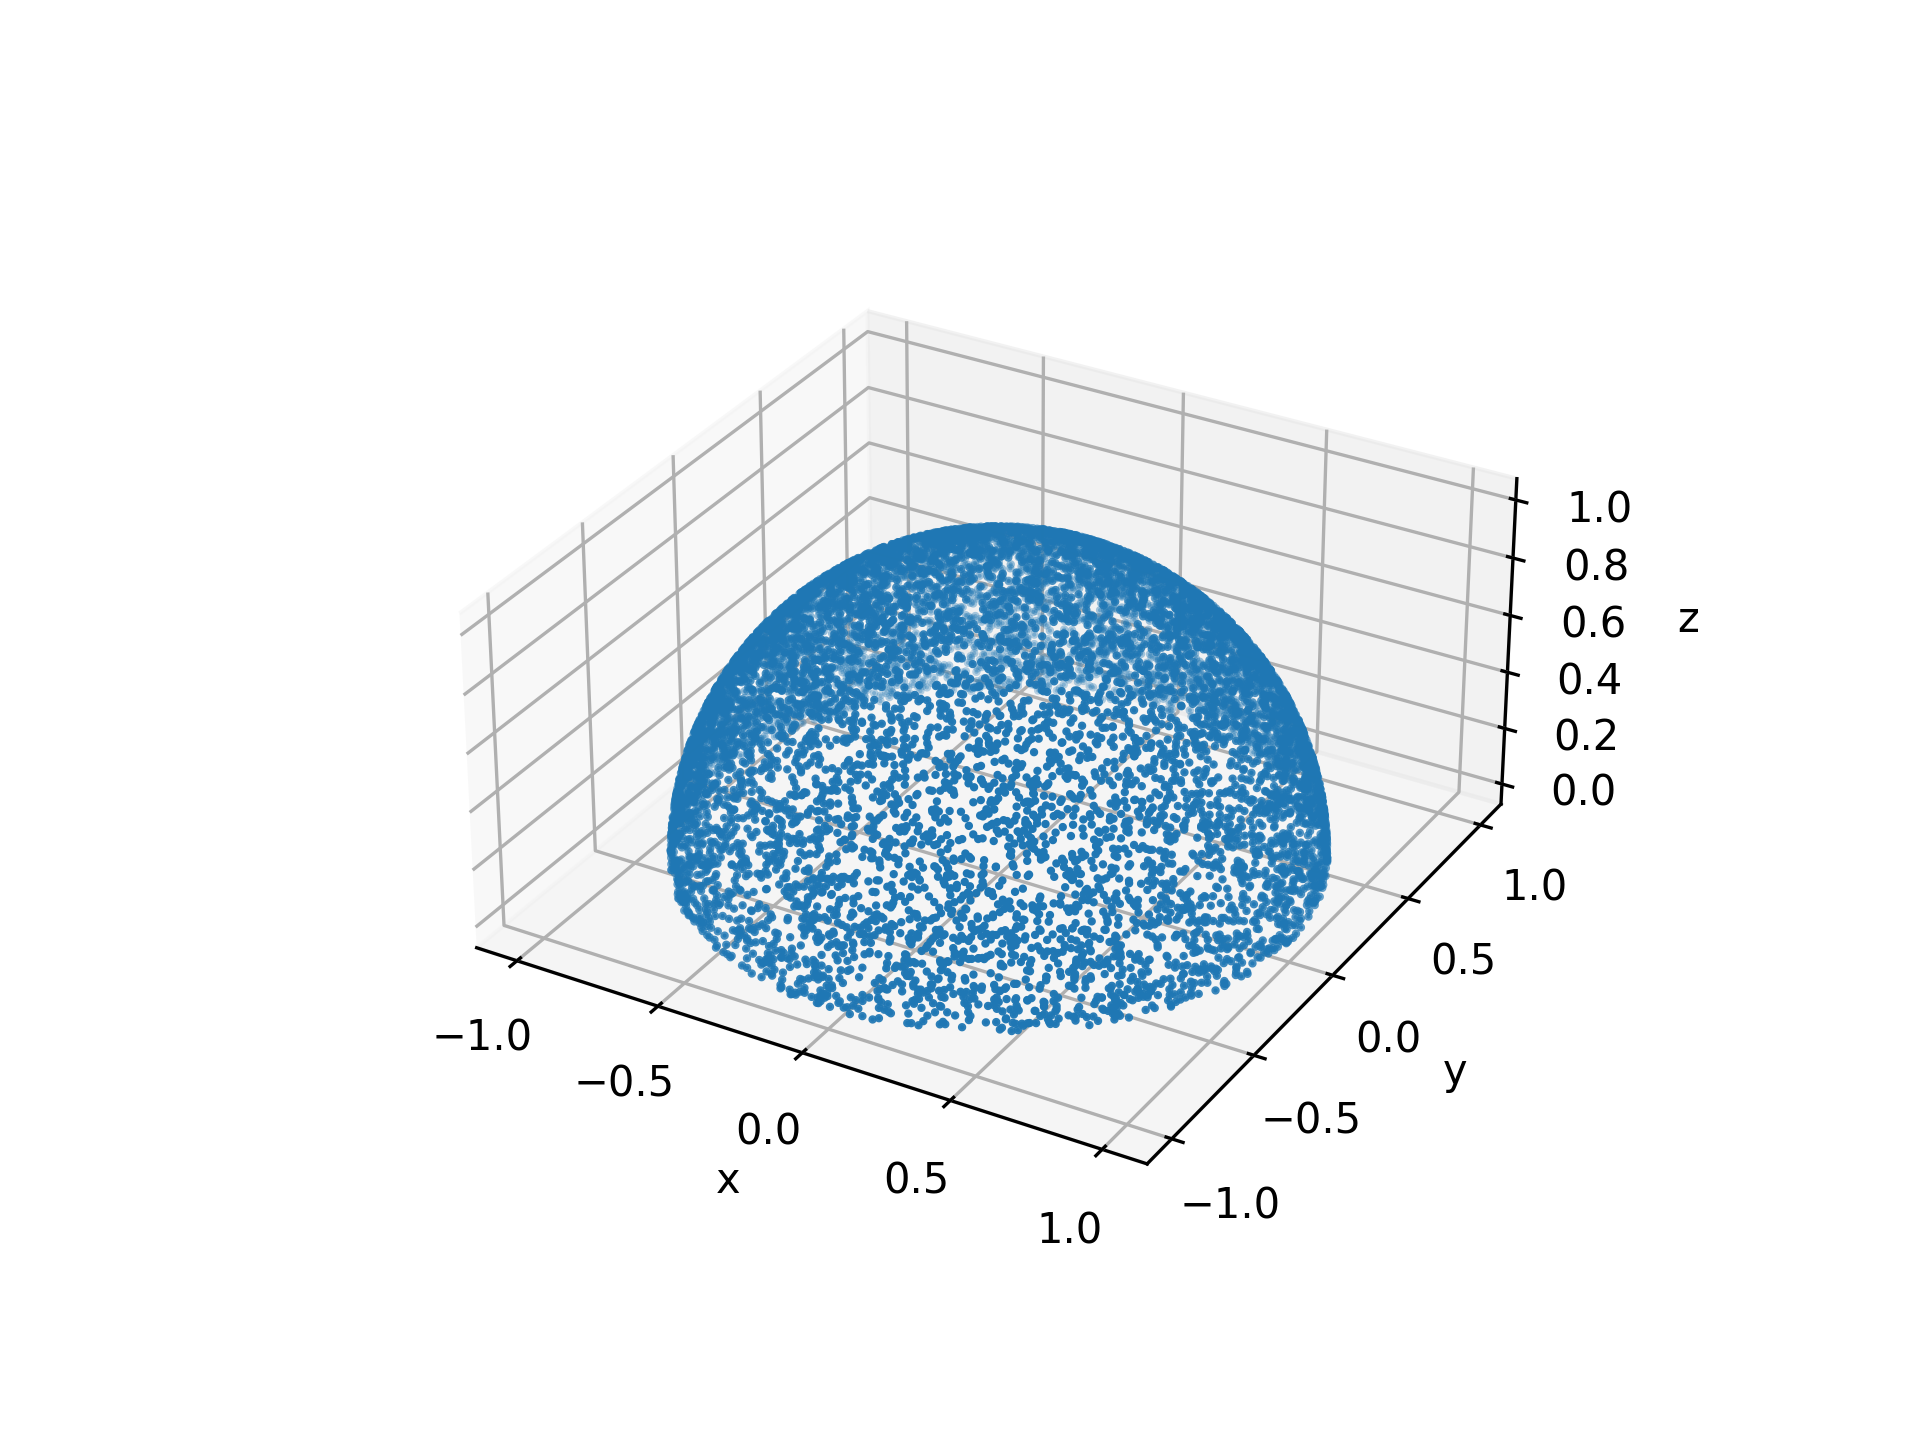
\includegraphics[width=0.48\textwidth]{fig4.eps}} \hfill
    \subfloat[783765个随机数点]{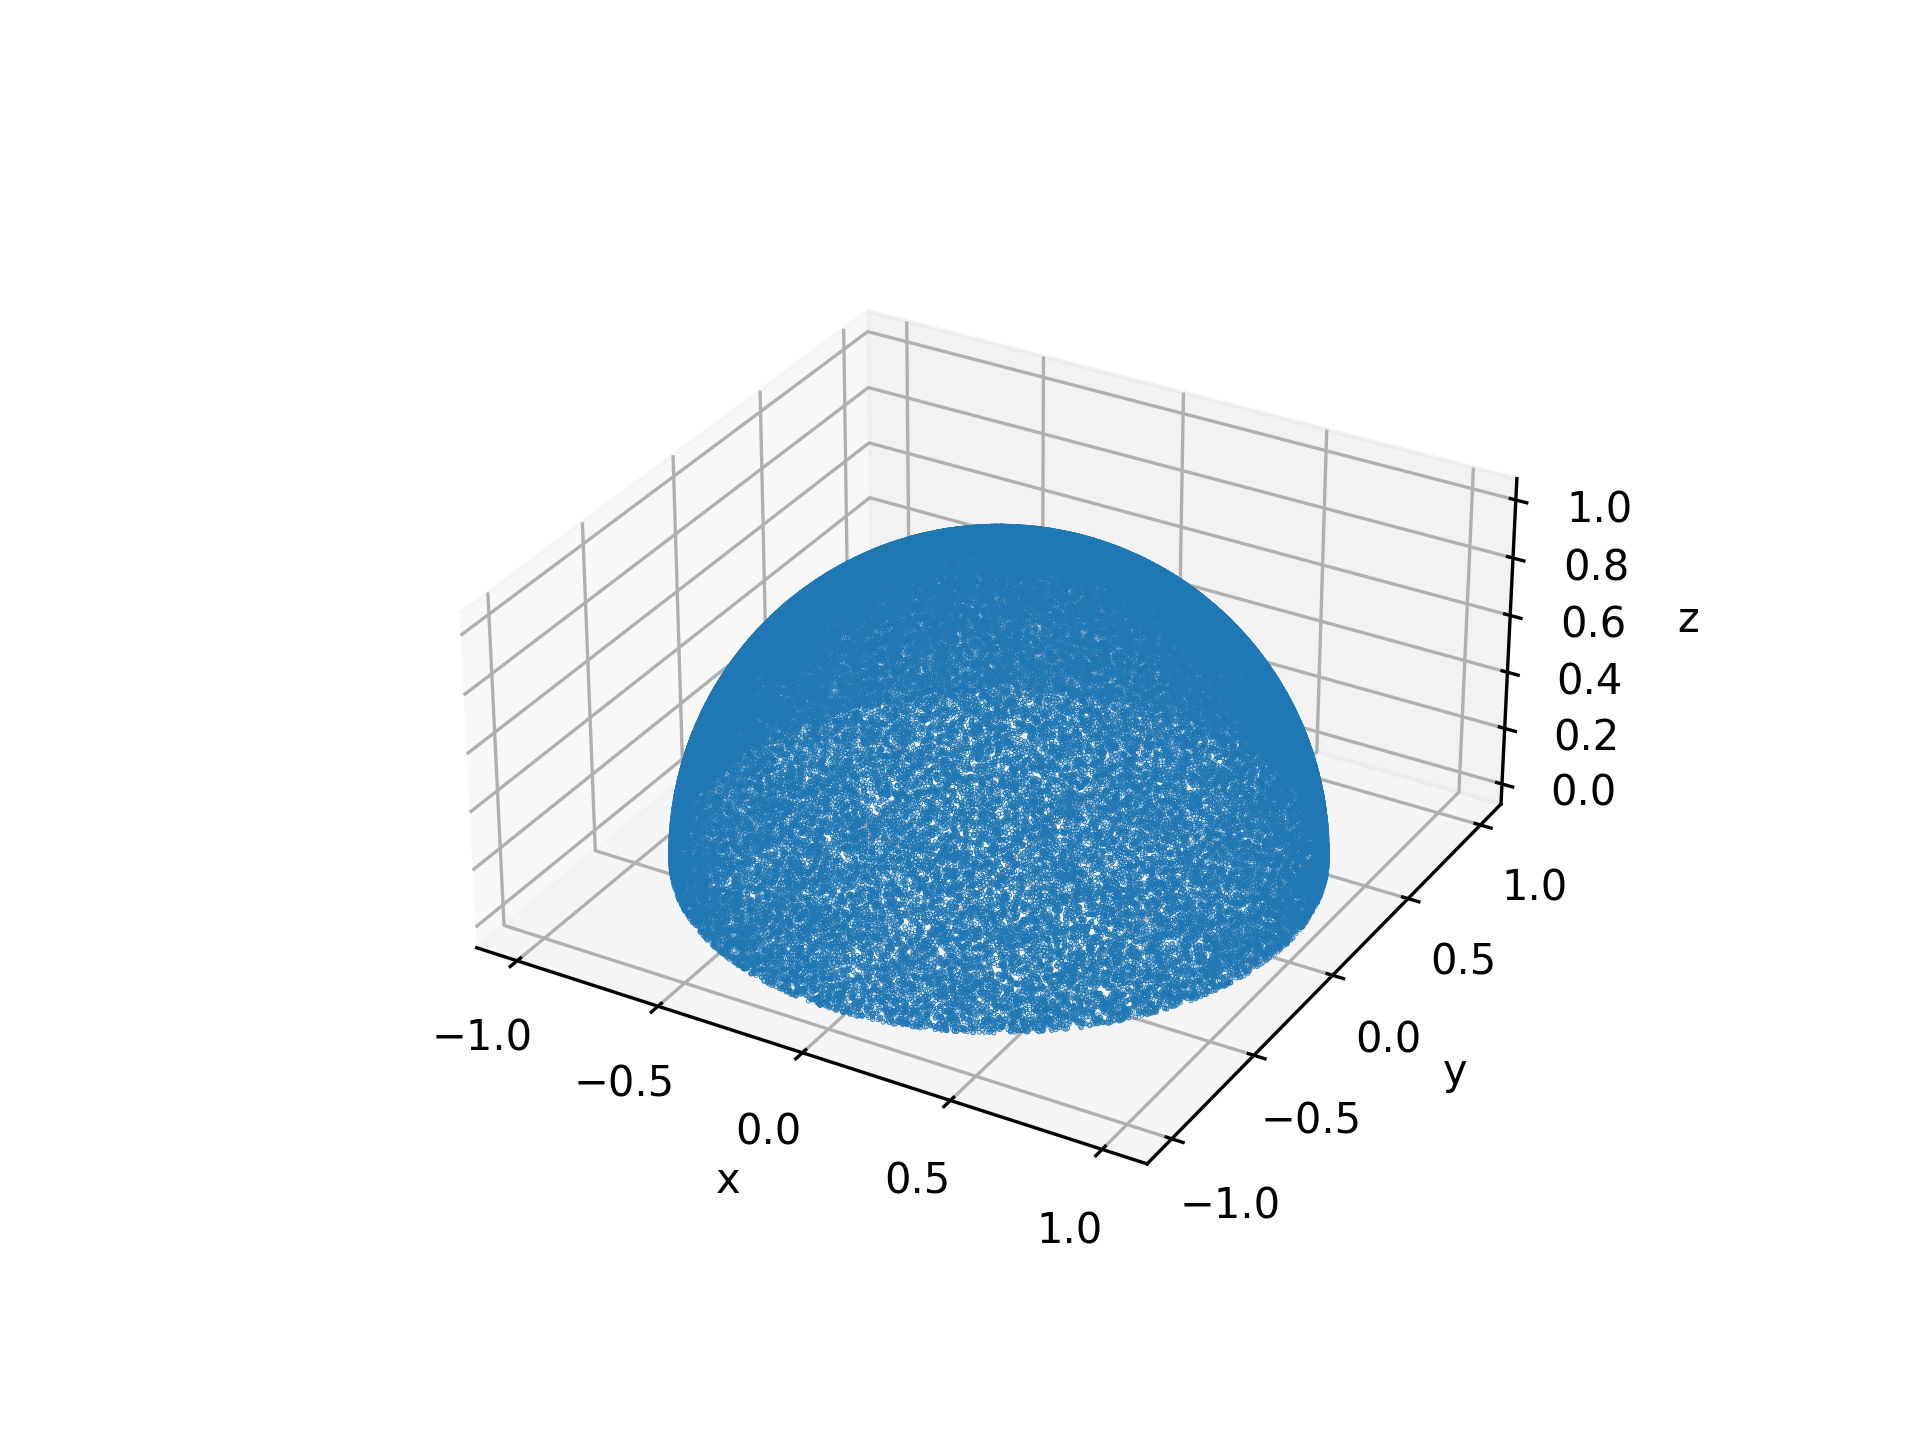
\includegraphics[width=0.96\textwidth]{fig5.eps}}
    \caption{Marsaglia抽样方法生成的随机数点散点图}
\end{figure}

\end{document}
